% !TEX root = ../main_lecture_notes.tex
% \chapter{Applications en mathématique financière}\label{chap:math_fi}
% Le contenu de ce chapitre s'inspire des notes de cours de \citet{Tankov2010} et de l'ouvrage de \citet{Mikosch1998}.
% \section{Un premier modèle de mathématique financière}
% \subsection{Notions de finance de marché}\label{sec:financial_market}
% les actifs financiers sont des produits échangeable sur les marché financiers, ils comprennent 
% \begin{itemize}
%     \item Les actions, il s'agit d'un titre de propriété partiel d'une entreprise (action d'entreprise du CAC40)
%     \item Les obligations (bond du trésors américain) 
%     \item les commodités (l'or, le pétrole, ...)
% \end{itemize}
% La valeur d'un actif au cours du temps est une suite de variable aléatoire $(S_t)_{t \geq 0}$, indicée sur le temps $t\geq0$.\\ 

% \noindent Un produit dérivé est un actif dont la valeur dépend de la valeur d'un autre actif financier, dit sous-jacent. Un produit dérivé commun sont les options, appelés \textit{put} et \textit{call} qui permettent l'achat ou la vente d'un titre à un prix fixé à l'avance. 
% \begin{definition}\label{def:eu_option}
% Une Option d'achat (resp. de vente) européenne donne le droit (pas l'obligation) d'acheter un titre à la date $T$ au prix $K$. Le flux de trésorerie (\textit{pay-off}) associé à ce contrat est donnée par 
% $$
% (S_T-K)_{+}\text{ (resp. }(K-S_T)_{+})
% $$ 
% \end{definition}
% \begin{itemize}
% \item Un marché financier permet l'échange d'actif financier et permet également d'emprunter du \textit{cash}. L'emprunt doit être rembourser à un taux d'intérêt $r$ correspondant au rendement d'actif dit non-risqué, c'est à dire soumis à pratiquement aucun aléa (typiquement les obligations d'état).
% \item Un portefeuille est une collection d'actif financier détenu par un investisseur
% \item Une opportunité d'arbitrage est une stratégie permettant de retirer un profit à partir d'un investissement initial nul. 
% \end{itemize}
% \begin{ex}
% Un contrat \textit{forward} est un produit dérivé sous la forme d'un contrat entre deux partie qui s'accorde pour acheter ou vendre un titre à $t>0$ au prix $F$. Si l'actif sous-jacent a une valeur initial $S_0$ alors le prix sans-arbitrage de ce contrat est 
% $$
% F = (1+r)^t S_0
% $$
% \begin{itemize}
%     \item Si $F > S_0(1+r)^t$. A $t = 0$, l'investisseur emprunte $S_0$ à la banque pour acheter le titre sous-jacent et propose un contrat de vente de l'actif au prix $F$ à date $t$. A la date $t$, il revend son actif au prix F et rembourse $S_0(1+r)^t$ à la banque en réalisant un profit 
%     $$
%     F-S_0(1+r)^t
%     $$ 
%     \item Si $F < S_0(1+r)^t$. A $t = 0$, l'investisseur emprunte l'actif au courtier et le revend immédiatement au prix $S_0$. Le montant $S_0$ est investit à la banque au taux $r$. Il propose un contrat forwward d'achat du sous-jacent au prix $
%     F$. A la date $t$, il achète l'actif au prix $F$, le rend au courtier. Il réalise ainsi un bénéfice 
%     $$
%     S_0(1+r)^t-F.
%     $$
% \end{itemize}
% \end{ex}

% L'objectif des mathématiques financières est de propopser des modèles pour les actifs permettant le calcul du prix des produits  dérivés en supposant une absence d'opportunité d'arbitrage. 

% \subsection{Le modèle binomial}\label{sec:binomial_modele}
% Soit $(S_t)_{t\geq 0}$ le prix d'un actif financier\footnote{\url{https://en.wikipedia.org/wiki/Financial_asset}} au cours du temps, par exemple le prix d'une action. 
% Il s'agit d'une suite de variables aléatoires indicée sur le temps $t\geq 0$, ce que nous appelerons processus stochastique dans la suite. L'actif dit risqué a une valeur initiale $S_0 = S$, et sa valeur à $t= 1$ est donnée par une variable aléatoire $S_1$ définie sur un espace probabilisé $(\Omega, \mathcal{F}, \mathbb{P})$, tel que 
% $$
% \Omega = (\omega_u,\omega_d),\text{ }0<\mathbb{P}(\{w_u\}) = p<1,\text{ et }\begin{cases}
% S_1(\omega_u) = uS,\\
% S_1(\omega_d) = dS,
% \end{cases}
% $$
% avec $s,u,d>0$ et $u>d$. L'évolution de l'actif risqué peut être représenté à l'aide d'un arbre, \cf \cref{fig:actif_risk}.
% \begin{figure}[h!]
% \begin{center}
% \begin{tikzpicture}[>=stealth,sloped]
%             \matrix (tree) [%
%             matrix of nodes,
%             minimum size=0.5cm,
%             column sep=3cm,
%             row sep=0.5cm,
%             ]
%         { &  & $su^2 $ \\
%  & $su $ &  \\
% $s$ &  & $su d$ \\
%  & $s d$ &  \\
%  &  & $s d^2$ \\
% };
% \draw[->] (tree-4-2) -- (tree-3-3) node [midway,above] {$ p (1-p) $};
% \draw[->] (tree-4-2) -- (tree-5-3) node [midway,above] {$  (1-p)^2 $};
% \draw[->] (tree-3-1) -- (tree-2-2) node [midway,above] {$ p  $};
% \draw[->] (tree-3-1) -- (tree-4-2) node [midway,above] {$  (1-p) $};
% \draw[->] (tree-2-2) -- (tree-1-3) node [midway,above] {$ p^2  $};
% \draw[->] (tree-2-2) -- (tree-3-3) node [midway,above] {$ p (1-p) $};
% \end{tikzpicture}
% \caption{Evolution de l'actif risqué}
% \label{fig:actif_risk}
% \end{center}
% \end{figure}
% \begin{remark}
% $(S_t)_{t\geq0}$ est une chaine de Markov homogène sur $\{u^id^js\}_{i,j\in\N}$ de matrice des transition 
% $$
% \mathbf{Q} =\left(\begin{array}{cc}p&0\\
% 0&1-p\end{array}\right) .
% $$
% \end{remark}
% Il y a également sur le marché un actif sans risque $(S^0_t)_{t\geq0}$ tel que $S^0_0 = 1$ et 
% $$
% S^0_1(\omega_u) = S^0_1(\omega_d) = \e^r = R.
% $$
% Il s'agit par exemple d'un livret d'épargne de taux d'intérêt $R>0$\footnote{$\text{d}S_t = r S_t\text{d}t$}.\\

% \noindent Une stratégie (auto-financée) est un couple $(x,\theta)\in \RL^2$, avec 
% $X$ le capital initial et $\theta$ le nombre de part d'actif risqué détenu sur la période $t\in[0, 1]$ La richesse au temps $t$ est donnée par 
% $$
% X_1 = (x-\theta S_0)R+ \theta S_1.
% $$
% On compare souvent la valeur actuelle des actifs et stratégie, le taux d'actualisation est donnée par le rendement de l'actif sans risque. On définit ainsi la valeur actuelle de l'actif risqué, de l'actif sans risque et de la stratégie $(x,\theta)$ par 
% $$
% \tilde{S}_1 = \frac{S_1}{\Delta},\text{ }\tilde{S}_1^0 = 1\text{, et }\tilde{X}_1 = x + \theta(\tilde{S}_1 - \tilde{S}_0).
% $$
% La valorisation financière des actifs repose sur l'hypothèse d'absence d'opportunité d'arbitrage. 

% \begin{definition}\label{def:opportunite_arbitrage}
% Une opportunité d'arbitrage est une stratégie $(0,\theta)$ telle que 
% $$
% X_1(\omega_i)\geq0,\text{ }i\in\{u,d\}\text{, et }\mathbb{P}(X_1>0)>0.
% $$

% \end{definition}
% \begin{prop}
% Dans notre modèle, l'absence d'opportunité d'arbitrage équivaut à 
% $$
% d<R<u.
% $$
% \end{prop}
% \begin{proof}
% \begin{itemize}
%     \item[(i)] Supposons que $R>u$. \\

%     A $t=0$, L'investisseur emprunte une part d'actif risqué au courtier et le revend immédiatement au prix $S_0 = s$. le montant $s$ est investit dans l'actif risqué.\\

%     A $t=1$, l'actif au prix est acheté au prix $S_1$ et rendu au courtier. Un profit positif est réalisé presque sûrement puisque
%     $$
%     X_1 = \begin{cases}
%     s(R-u),&\text{ si }\omega_u,\\
%     s(R-d),&\text{ si }\omega_d.
%     \end{cases}
%     $$ 
%     \item[(ii)] Supposons que $R<d$.\\

%     A $t=0$, L'investisseur emprunte $S_0 = s$ à la banque pour acquérir une part d'actif risqué.\\ 

%     A $t=1$, l'actif est revendu $S_1$ le montant $sR$ est remboursé au banquier. Un profit positif est réalisé presque sûrement puisque
%     $$
%     X_1 = \begin{cases}
%     s(u-R),&\text{ si }\omega_u,\\
%     s(u-R),&\text{ si }\omega_d.
%     \end{cases}
%     $$
% \end{itemize}
% \end{proof}
% Un produit dérivé est un contrat dont le \textit{pay-off} $V$ dépend de l'actif risqué sous-jacent, par exemple dans le cas d'un call européen de maturité $1$ et de prix d'exercice $K$, on a $V = (S_1-K)_+$. Il est possible de répliquer le \textit{pay-off} $V$ à l'aide d'une stratégie auto-financé. Il s'agit de trouver le couple $(x,\theta)$ tel que 
% $$
% \begin{cases}
% V(\omega_u) = \theta u S_0+R(x-\theta S_0)
% V(\omega_d) = \theta d S_0+R(x-\theta S_0)
% \end{cases}.
% $$
% On en déduit que 
% $$
% \theta = \frac{V(\omega_u)-V(\omega_d)}{S_0(u-d)}
% $$
% et 
% \begin{equation}\label{eq:valeur_initiale}
% x=\frac{V(\omega_u)}{R}\frac{R-d}{u-d} + \frac{V(\omega_d)}{R}\frac{u-R}{u-d}
% \end{equation}
% Soit $q =\frac{R-d}{u-d}$, en l'absence d'opportunité d'arbitrage $q\in(0,1)$. On définit une mesure de probabilité $\Q$, équivalente à $\Prob$, telle que 
% $$
% \Q(S_1 = uS_0) = q\text{ et }\Q(S_1 = dS_0) = 1-q.
% $$ 
% Le prix du produit dérivé est donné par son espérance (à la manière d'une prime en assurance). Sous la probabilité $\Q$, le prix est exactement l'investissement initial du portefeuille répliquant $x = \mathbb{E}_{\Q}(\tilde V)$. Sous cette probabilité encore, on a 
% $$
% \mathbb{E}_\Q(S_1) = RS_0.
% $$
% Cela signifie que, sous la probabilité risque neutre, le rendement moyen de l'actif risqué est le même que celui de l'actif non risqué. Il est possible que sous la probabilité historique $\mathbb{E}_\Prob(S_1) \geq RS_0$\ (\textit{higher risk, higher gain} pour inciter les agents à investir dans l'actif risqué!). 
% On remarque aussi que
% $$\mathbb{E}_\Q(\tilde{S}_1) = S_0.
% $$ 
% Le processus $(\tilde{S}_t)_{t\geq0}$ est donc une $\Q-$martingale. La mesure de probabilité $\mathbb{Q}$ est la probabilité risque neutre. Son existence et son unicité sont équivalente à l'absence d'opportunité d'arbitrage. 
% \begin{remark}
% La tarification des produits dérivés doit s'effectuer suivant la probabilité risque neutre sans quoi il existe une opportunité d'arbitrage. 
% \begin{itemize}
%     \item Supposons que $x > \mathbb{E}_{\Q}(V)$
%     \begin{itemize}
%         \item A $t=0$, J'emprunte $\theta S_0$ au courtier et $x-\theta S_0$ à la banque. je revend immédiatement $\theta S_0$. J'ai un capital initiale de $x$. J'achète le produit dérivé au prix $\E_{\Q}(\tilde V)$ et je place $(x-\E_{\Q}(\tilde V)$ sur mon compte épargne.  
%         \item A t = 1, je reçois $V = \theta S_1 + (x-\theta S_0)R $. Je rembourse mon prêt à la banque $(x-\theta S_0)R$, j'achète l'actif risqué au prix $\theta S_1$ que je rend au courtier. Il me reste $(x-\mathbb{E}_\Q(\tilde V))R > 0$
%     \end{itemize}
%     \item Supposons que $x < \mathbb{E}_{\Q}(V)$
%     \begin{itemize}
%         \item A $t=0$, Je vends le produit dérivé au prix $\E_{\Q}(\tilde V)$. Je place $x-\theta S_0$ à la banque et j'achète $\theta S_0$ au courtier. Je place $\E_{\Q}(\tilde V)-x$ à la banque. 
%         \item A t = 1, Mon investissement rapport $V + (\E_{\Q}(\tilde V)-x)R$ et je cède $V$ à l'acheteur du produit dérivé. Il me reste $(\mathbb{E}_\Q(\tilde V)-x)R > 0$
%     \end{itemize}
% \end{itemize}
% L'équilibre sur le marché des produits dérivés suppose que la tarificaation a été effectué sous la mesure de probabilité risque neutre, le taux d'actualisation à utiliser $R$ doit permettre de vérifier la propriété "martingale" de la valeurs des actifs sous jacents. Ici on suppose que ce taux sans-risque $R$ est calibré sur la base des prix correspondant à un équilibre offre et demande ayant gommer les opportunités d'arbitrage.
% \end{remark}

% \subsection{Le modèle de Cox-Ross-Rubinstein}
% Soit $T>0$ un horizon de temps et $i\frac{T}{N}, i = 0,\ldots,N$ une subdivision de $[0, T]$. Soit $(S_n)_{n\leq N}$ la valeur de l'actif sous jacent dont la dynamique est donnée par 
% $$
% S_n = S_0\exp(n\mu_N + Z_n\sigma_N), n = 0,\ldots, N. 
% $$
% où $\mu_N = \mu\frac{T}{N}$, $\sigma_N = \sigma\sqrt{\frac{T}{N}}$, et $Z_n = \sum_{i = 1}^n\xi_i$, avec des $\xi_i$ \iid suivant la loi
% $$
% \mathbb{P}(\xi_i=1) = p\text{ et }\mathbb{P}(\xi_i=1) = 1-p,
% $$
% et $Z_0 = 0$
% \begin{remark}
% \begin{enumerate}
%     \item Le processus $Z$ est une marche aléatoire sur $\mathbb{Z}$. Il s'agit d'une chaine de Markov homogène,  irréductible, récurrente si $p = 1/2$, de noyau de transition
%     $$
%     \mathbb{P}(Z_{n} = y|Z_{n} = x) = Q(x,y) = \begin{cases}
%     p, &\text{ si }y = x+1, \\
%     1 - p,&\text{ si }y = x-1, \\
%     0, &\text{ sinon, }\\
%     \end{cases}\text{ pour tout }n\geq1.
%     $$ 
%     \item  Le processus $S$ est aussi une chaine de Markov, on peut écrire 
%     $$
%     S_n = S_{n-1}\exp(\mu_N + \xi_{n}\sigma_N),\text{ pour tout }n\geq1.
%     $$
% \end{enumerate}

% \end{remark}
% Ce modèle est équivalent au modèle binomial avec
% $$
% u_N = e^{\mu_N + \sigma_N}\text{ et }d_N = e^{\mu_N - \sigma_N}.
% $$
% Le rendement des actifs est souvent défini par $S_n / S_{n-1}$, les log rendements vérifient 
% $$
% \mathbb{E}[\ln(S_n / S_{n-1})] = \mu_N\text{ et }\mathbb{V}[\ln(S_n / S_{n-1})] = \sigma_N^2
% $$
% $\mu_N$ est le drift et $\sigma_N$ la volatilité. Le rendement de l'actif sans risque sur une période de temps de longueur $T/N$ est donné par $R_N = e^{rT/N}$. La \cref{fig:traj_CRR} montre des trajectoires de l'actif risqué et de l'actif sans risque.
% \begin{figure}
% \centering
% 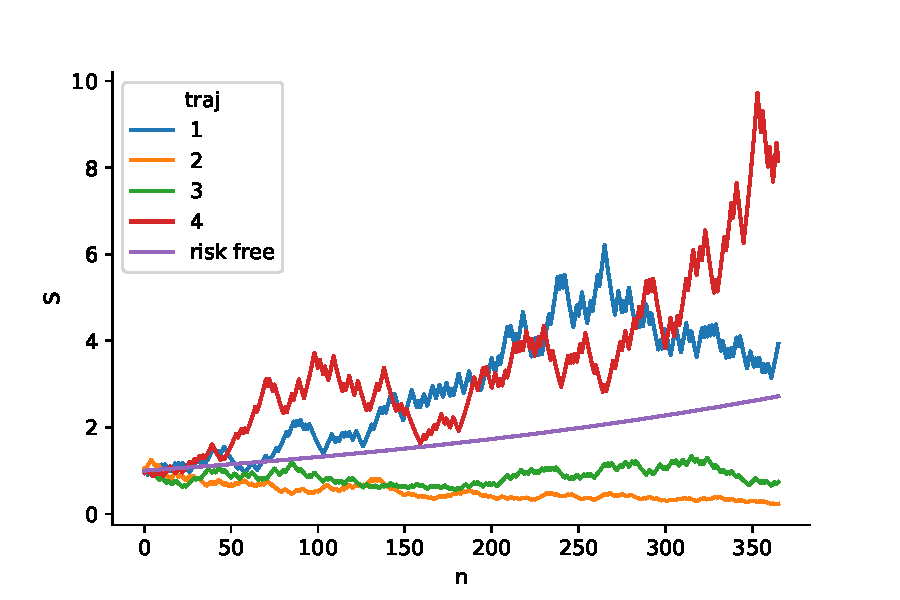
\includegraphics[width = \textwidth]{../Figures/traj_CRR.pdf}
% \caption{Trajectoires du processus $S$ et de l'actif sans risque}
% \label{fig:traj_CRR}
% \end{figure}

% Par analogie avec le modèle binomial, sous la probabilité risque neutre $\Q$, le processus $\tilde{S}_n = S_n/R_N^n,\text{ }n\geq0$ est une $\Q-$martingale. Les variables aléatoires $S_n$ sont mesurable par rapport à la tribu engendrée par les $\xi_i,\text{ }i\leq n$, noté $\mathcal{F}_n = \sigma_N(\xi_1,\ldots, \xi_n)$. La suite $(\F_n)_{n\geq0}$ est une suite de sous-tribu croissante pour l'inclusion que l'on appelle filtration du processus $S$. Il s'agit de l'information détenue sur le processus jusqu'à l'instant $n$. Le processus $\tilde S$ est une $\Q$-martingale s'il vérifie 
% $$
% \E_\Q(\tilde{S}_n|\F_{n-1}) =  \tilde S_{n-1}.
% $$
% On observe que 
% \begin{eqnarray*}
% \E_\Q(\tilde{S}_n|\F_{n-1})& =& \E_\Q\left[\frac{S_{n-1}}{R_N^n}\e^{\mu_N + \xi_{n}\sigma_N}|\F_{n-1}\right]\\
% & =& \frac{S_{n-1}}{R_N^n}\e^\mu_N\E_\Q\left[\e^{\xi_{n}\sigma_N}|\F_{n-1}\right]\\
% & =& \tilde S_{n-1}\frac{\e^\mu_N}{R_N}\E_\Q\left[\e^{\xi_{n}\sigma_N}\right]\\
% & =& \tilde S_{n-1}\frac{q\e^{\mu_N+\sigma_N}+ (1-q)\e^{\mu_N-\sigma_N} }{R_N}\\
% \end{eqnarray*}
% Pour que $S$ soit une martingale, il faut que 
% $$
% q\e^{\mu_N+\sigma_N}+ (1-q)\e^{\mu_N-\sigma_N} = R_N \Leftrightarrow q = \frac{R_N-\e^{\mu-\sigma_N}}{\e^{\mu+\sigma_N}-\e^{\mu_N-\sigma_N}}.
% $$
% On a bien identifié la probabilité risque neutre $\Q$ telle que 
% $$
% \Q(\xi = 1) = \frac{R-e^{\mu_N-\sigma_N}}{\e^{\mu_N+\sigma_N}-\e^{\mu_N-\sigma_N}}=\frac{R_N-d_N}{u_N-d_N}=q_N
% $$
% de manière analogue au modèle binomial. La valorisation d'un produit dérivé $g(S_n)$ se fait sous la probabilité risque neutre avec 
% $$
% \pi = e^{-rT}\mathbb{E}_\Q[g(S_N)].
% $$ 
% Cette espérance se calcule bien en remarquant que 
% $$
% \Q\left(S_N = S_0u_N^kd_N^{N-k}\right) = \binom{N}{k}q_N^k(1-q_N)^{N-k},\text{ pour }k = 0,\ldots, N.
% $$
% Prenons l'exemple du call européen avec $g(s) = (s-K)_+$. Soit 
% \begin{equation}\label{eq:eta}
% \eta_N =\inf\{k = 0,\ldots, N\text{ ; }S_0u_N^kd_N^{N-k}>K\},
% \end{equation}
% et $\bar{F}(n,p,k) = \Prob[\BinomialDist(n,p)> k]
% $. On a 
% \begin{equation}\label{eq:price_call_Binomial}
% \pi_N = R_N^{-N}\mathbb{E}_\Q[(S_N-K)_+] = S_0\bar{F}(N,\frac{q_Nu_N}{R_N},\eta_N)- e^{-rT}K \bar{F}(N,q_N,\eta_N).
% \end{equation}
% Le modèle de Cox-Ross-Rubinstein est une approximation d'un modèle en temps continu obtenu en laissant $N$ tendre vers l'infini. On note que sous la probabilité historique $\Prob$ et avec $p=1/2$, il vient
% $$
% \log\left(\frac{S_N}{S_0}\right) = N\mu_N+Z_N\sigma_N = \mu T + \frac{Z_N}{\sqrt{N}}\sigma\sqrt{T}\overset{\text{TCL}}{\sim}\NormalDist(\mu T, \sigma^2T)
% $$
% Les log rendements gaussien sont une caractéristique du modèle de Black-Scholes qu'on étudiera par la suite. Faire tendre $N$ vers l'infini permet également d'approcher le prix du call $\eqref{eq:price_call_Binomial}$. On a besoin du résultat suivant. 

% \begin{lemma}
% Soit $(X_n)_{n\geq0}$ une suite de \va indépendantes tel que $X_k\sim\BinomialDist(k, p_k)$ pour $k\geq1$ t alors 
% $$
% \frac{X_n-np_n}{\sqrt{np_n(1-p_n)}}\overset{\mathcal{D}}{\rightarrow}\NormalDist(0,1), \text{ lorsque }n\rightarrow\infty
% $$
% \end{lemma}
% \begin{proof}
% On montre que 
% $$
% \underset{n\rightarrow \infty}{\lim} \E(e^{tX_n})= \e^{t^2/2}.
% $$
% \end{proof}
% D'après la définition de $\eta_N$, voir \eqref{eq:eta}, on a l'encadrement
% $$
% S_0u_N^{\eta_n-1}d_N^{N-\eta_n+1}\leq K\leq S_0u_N^{\eta_n}d_N^{N-\eta_n}.
% $$
% On en déduit en passant au log que  
% $$
% \eta_N\sigma\frac{\sqrt{T}}{\sqrt{N}} + N\left(\mu\frac{T}{N} - \sigma\frac{\sqrt{T}}{\sqrt{N}}\right) =\ln(K/S_0)+o(\sqrt{N})
% $$
% puis
% $$
% \eta_N = \frac{N}{2}+\frac{\sqrt{N}}{2\sigma\sqrt{T}}\left[\log(K/S_0)-\mu T\right]+ o(\sqrt{N})\text{, lorsque }N\rightarrow\infty.
% $$
% On a également
% $$
% q_{N} = \frac{e^{r\frac TN}-e^{\mu\frac TN-\sigma\sqrt{\frac{T}{N}}}}{e^{\mu\frac TN+\sigma\sqrt{\frac TN}} - e^{\mu\frac TN-\sigma\sqrt{\frac{T}{N}}}}
% $$
% Un développement limité à l'ordre 1 permet de conclure que $q_N\rightarrow 1/2$ pour $N\rightarrow +\infty$. Un développement limité à l'ordre 2 permet d'observer que 
% $$
% Nq_N = \frac{N}{2}+\frac{(r-\mu-\sigma^2/2)T}{2\sigma\sqrt{T}}\sqrt{N} + o(\sqrt{N})
% $$
% et de conclure que 
% $$
% \frac{\eta_N - Nq_N}{\sqrt{Nq_N(1-q_N)}} \rightarrow \frac{1}{\sigma\sqrt{T}}\left[\log(\widetilde{K}/S_0) + \sigma^2/2\right]= d^+,
% $$
% où $\widetilde{K} = Ke^{-rT}$. On a également 
% $$
% \frac{q_Nu_N}{R_N} = \frac{e^{r\frac TN}-e^{\mu\frac TN-\sigma\sqrt{\frac{T}{N}}}}{e^{\mu\frac TN+\sigma\sqrt{\frac TN}} - e^{\mu\frac TN-\sigma\sqrt{\frac{T}{N}}}}
% \cdot 
% \frac{e^{\mu\frac TN+\sigma\sqrt{\frac{T}{N}}}}{e^{r\frac TN}} = 
% \frac{e^{(r+\mu)\frac TN+\sigma\sqrt{\frac TN}}-e^{2\mu\frac TN}}{e^{(r+\mu)\frac TN+\sigma\sqrt{\frac TN}} - e^{(r+\mu)\frac TN-\sigma\sqrt{\frac{T}{N}}}}
% $$
% Ce qui permet d'affirmer que 
% $$\frac{q_Nu_N}{R_N}\rightarrow 1/2\text{, et }
% N\frac{q_Nu_N}{R_N} = \frac{N}{2}+\frac{(r-\mu+\sigma^2/2)T}{2\sigma\sqrt{T}}\sqrt{N} + o(\sqrt{N})\text{ lorsque } N\rightarrow +\infty.
% $$
% Il vient alors 
% $$
% \frac{\eta_N - Nq_Nu_N/R_N}{\sqrt{Nq_Nu_N/R_N(1-q_Nu_N/R_N)}} \rightarrow \frac{1}{\sigma\sqrt{T}}\left[\log(\widetilde{K}/S_0) - \sigma^2/2\right] = d^-. 
% $$
% On conclut que 
% $$
% \pi_N\approx S_0[1-\phi(d^-)]- \widetilde{K} [1-\phi(d^+)].
% $$
% où $\phi(\cdot)$ est la fonction de répartition de la loi normal centrée réduite. On vérifie avec Python!
% \section{Le modèle de Black-Scholes-(Merton)}\label{sec:BS}
% \subsection{Le Set up}
% Soit une économie comprenant deux actifs l'un risqué, l'autre non. Le prix de l'actif risqué (action ou indice boursier) est un processus $S$ défini sur un espace probabilisé filtré $(\Omega,\F, \F_t, \Prob)$ dont la dynamique est donnée 
% par 
% $$
% \text{d}S_t = \mu \text{d}t + \sigma \text{d}B_t,
% $$ 
% où $(B_t)_{t\geq 0}$ est un mouvement brownien standard indépendant de $S_0$ la position initiale de $X$. Par application de la formule d'Ito sur $\ln S_t$, nous obtenons 
% $$
% S_t = S_0\exp[(\mu - \sigma^2/2)t + \sigma B_t],\text{ }t\geq 0.
% $$
% De son côté l'actif sans risque (bond du trésor américain ou livret A) admet une dynamique déterministe avec 
% $$
% \di S_t^0 = r S_t^0 \di t.
% $$
% où $r>0$ désigne le rendement de l'actif sans risque. En supposant que $S^0_0 = 1$, il vient 
% $$
% S_t^0 = \e^{r t}. 
% $$
% Un portefeuille contient contient à l'instant $t\geq 0$ une certaine part d'actif risqué et d'actif non-risqué. Soit $(a_t)_{t\geq 0}$ et $(b_t)_{t\geq 0}$ deux processus $\F_t$-adapté égale au nombre d'unité d'actif risqué et d'actif sans risque contenu dans le portefeuille. La valeur du portefeuille est donnée par 
% $$
% V_t = a_t S_t + b_t S^0_t,\text{ }t\geq 0.
% $$
% le couple $(a_t, b_t)_{t\geq 0}$ est une stratégie d'investissement. Nous supposons que la stratégie d'investissment est \textit{auto-finançante}, c'est à dire que les fluctuations de la valeur du portefeuille ne sont dues qu'aux fluctuations des prix des actifs. Cette hypothèse se traduit par 
% $$
% \di V_t = a_t \di S_t + b_t \di S^0_t = (a_t\mu S_t + b_tr S_t^0)\di t  + a_t \sigma S_t \di B_t.
% $$
% Nous souhaitons donner un prix juste à une option européenne de maturité $T$ et de prix d'exercice $K$. Selon Black, Scholes and Merton, la valeur juste est défini par deux hypothèses
% \begin{itemize}
%     \item L'existence d'une stratégie autofinançante permettant la réplication exacte du \textit{pay-off} de l'option. 
%     \item Si l'option était vendu à un prix autre que le prix juste alors il y aurait une opportunité d'arbitrage, soit La possibilité d'un profit infini sans aucune prise de risque.
% \end{itemize}
% \subsection{La formule de Black-Scholes}
% Prenons l'exemple d'un call européen pour lequel la \textit{pay-off} à maturité est donné par 
% $$
% (S_T-K)_+.
% $$
% L'objectif est de déterminer une stratégie autofinançante telle que 
% $$
% V_t = a_t S_t + b_t S^0_t = u(T-t, S_t),\text{ }t\in [0, T],
% $$
% où $u(\cdot, \cdot)$ est une fonction régulière qui vérifie la condition terminale 
% $$
% V_T = u(0,S_T) = (S_T-K)_+.
% $$
% On applique la formule d'Ito pour obtenir 
% $$
% \text{d}V_t = \left[-\frac{\partial}{\partial t}u(T-t, S_t) + \mu S_t\frac{\partial}{\partial x}u(T-t, S_t) + \frac{\sigma^2 S_t^2}{2}\frac{\partial^2}{\partial x^2}u(T-t, S_t)\right]\text{d}t + \sigma S_t\frac{\partial}{\partial x}u(T-t, S_t)\text{d}B_t.
% $$
% On se rappelle que du fait du caractère auto-finançant de la stratégie d'investissement alors
% $$
% \di V_t = (a_t\mu S_t + b_tr S_t^0)\di t  + a_t \sigma S_t \di B_t.
% $$
% De plus comme $V_t = a_t S_t + b_t S^0_t$ alors 
% $$
% b_t = \frac{V_t - a_t S_t}{S^0_t}
% $$
% et 
% $$
% \di V_t = (a_t(\mu - r)S_t + V_t r )\di t  + a_t \sigma S_t \di B_t.
% $$
% On en déduit que 
% $$
% a_t = \frac{\partial}{\partial x}u(T-t, S_t),
% $$
% et 
% \begin{equation*}
% \frac{\partial}{\partial x}u(T-t, S_t)(\mu - r)S_t + r u(T-t, S_t) = -\frac{\partial}{\partial t}u(T-t, S_t) + \mu S_t\frac{\partial}{\partial x}u(T-t, S_t) + \frac{\sigma^2 S_t^2}{2}\frac{\partial^2}{\partial x^2}u(T-t, S_t)
% \end{equation*}
% Cette dernière égalité est en fait une équation aux dérivées partielles
% \begin{equation}\label{eq:edp_BS}
% \frac{\partial}{\partial x}u(t, x)(\mu - r)x + r u(t, x) = -\frac{\partial}{\partial t}u(t, x) + \mu x\frac{\partial}{\partial x}u(t, x) + \frac{\sigma^2 x^2}{2}\frac{\partial^2}{\partial x^2}u(t, x),
% \end{equation}
% vérifiée pour $x>0$ et $t\in[0,T]$, avec la condition terminale 
% $$
% u(0,x) = (x-K)_+.
% $$
% L'équation \eqref{eq:edp_BS} admet une solution explicite (quelle chance). En effet, 
% $$
% u(t,x) = x\phi(g(t,x)) - K\e^{-rt}\phi(h(t,x)),
% $$
% où $\phi$ est la fonction de répartition de la loi normale centrée réduite, 
% $$
% g(t,x) = \frac{\log(x/K) + (r+\sigma^2/2)t}{\sigma \sqrt{t}},
% $$
% et 
% $$
% h(t,x) = g(t,x) - \sigma\sqrt{t}.
% $$
% Le prix juste pour notre option européenne est donnée par 
% $$
% V_0 = u(T, X_0) = X_0\phi(g(T,X_0)) - K\e^{-rt}\phi(h(T,X_0)).
% $$
% C'est la formule que l'on retrouve dans les papiers de \citet{Black1973} et \citet{Merton1973}. La stratégie d'investissemnt permettant la réplication du \textit{pay-off} st donnée par 
% $$
% a_t = \frac{\partial}{\partial x}u(T-t, S_t),
% $$
% et 
% $$
% b_t = \frac{u(T-t, X_t) - a_t X_t}{S^0_t}.
% $$
% Pour comprendre la signification du prix juste $q = u(T, X_0)$ en terme d'arbitrage, supposons que l'option soit vendu au prix $p>q$. On applique la stratégie suivante: à $t=0$
% \begin{itemize}
%     \item Je vends l'option au prix $p$, 
%     \item J'investis $q$ dans la stratégie auto-finançante
% \end{itemize}
% Je dégage un profit initial $p-q$. A maturité si $X_T> K$ alors l'acheteur exerce l'option et ma stratégie autofinançante compense la perte $X_T-K$, sinon l'acheteur n'exerce pas l'option. Je peux dégagé un profit arbitrairement grand en supposant en vendant une grande quantité d'options.
% \subsection{Interprétation via la probabilité risque-neutre}
% Nous donnons une intéprétation du juste prix du call européen dans le cadre du modèle de Black-Scholes via un changement de mesure et le théorème de Girsanov. Un prix de départ raisonable est la valeur du flux de trésorie future actualisé au taux de l'actif sans risque soit
% $$
% \e^{-rT}(X_T - K)_+ = \e^{-rT}h(S_T)
% $$
% Le prix juste ne correspond pas à l'espérance du flux futur actualisé en tout cas pas sous la probabilité $\Prob$ dite historique. Il faut introduire une autre probalité dite risque neutre $\Q$. Dans la section précédente, cette probabilité était telle que le prix de l'actif actualisé était une martingale. Nous devons donc définir une probabilité pour laquelle le processus 
% $$
% \tilde{S}_t = \e^{-rt}S_t,\text{ }t\geq 0,
% $$
% est une $\Q$-martingale. Par application de la formule d'Ito, il vient 
% $$
% \text{d}\tilde{S}_t = \tilde{S}_t (\mu- r)\text{d}t + \tilde{S}_t \sigma\text{d}B_t.
% $$
% On définit $\tilde{B}_t = B_t - \frac{\mu - r}{\sigma}t,\text{ }t\geq0$. D'après le théorème de Girsanov $(\tilde{B}_t)_{t\geq 0}$ est un mouvement brownien sous la probabilité $\Q$ définie par 
% $$
% \Q(A) = \E_\Prob(Z_T^\theta\ind_A),
% $$
% où $Z_T^\theta = \e^{\theta B_t  - \theta t}$, et $\theta = \frac{\mu - r}{\sigma}.$ Le processus $(\tilde{S}_t)_{t\geq 0}$ dont la dynamique est donnée par 
% $$
% \text{d}\tilde{S}_t = \sigma\tilde{S}_t\text{d}\tilde{B}_t,
% $$
% est une $\Q$-martingale. Si on suppose qu'il existe une stratégie auto-finançante telle que 
% $$
% V_t = a_t S_t + b_t\beta_t
% $$
% tel que $V_T = h(S_T)$ alors la valeur du portefeuille à $T$ actualisée au temps $t$ est donnée par 
% $$
% \E(\e^{-r(T-t)}h(S_T)|\F_t),\text{ }t\in [0,T].
% $$
% Soit 
% $$
% \tilde{V_t} = \e^{-rt}V_t,\text{ }t\geq 0,
% $$
% la valeur actualisé du portefeuille. Par application de la formule d'Ito, il vient 
% \begin{eqnarray*}
% \text{d}\tilde{V_t}  &=& -r\e^{-rt}V_t\text{d}t + \e^{-rt}\text{d}V_t\\
%  &=&-r\e^{-rt}(a_t S_t + b_tS_t^0)\text{d}t + \e^{-rt}(a_t S_t + b_tS_t^0 ))\\
%  &=&a_t(-r\e^{-rt}S_t\text{d}t + \e^{-rt}\text{d}S_t)\\
%  &=&a_t\text{d}\tilde{S}_t
% \end{eqnarray*}
% Le processus est une $\Q$-martingale et donc 
% $$
% V_t = \E^\Q(\tilde{V}_T|\F_t),\text{ }t\in [0,T].
% $$
% On en déduit que 
% $$
% V_t = \E^\Q(\e^{-r(T-t)}h(X_T)|\F_t),\text{ }t\in [0,T].
% $$
% La dynamique de $(X_t)_{t\geq 0}$ est donnée par 
% $$
% \di X_t = r \di t + \sigma\di  \tilde{B}_t,
% $$
% et donc 
% $$
% X_t = X_0 \e^{(r-\sigma^2 / 2)t + \sigma \tilde{B}_t }.
% $$

% On a alors 
% $$
% V_t = f(t, X_t) = \E^\Q\left[\e^{-r(T-t)}h(X_t\e^{(r-\sigma^2 / 2)(T)-t + \sigma (\tilde{B}_T - \tilde{B}_t})|\F_t\right],
% $$
% qui est l'espérance d'une fonction d'une variable aléatoire $\NormalDist(0,T-t)$. On vérifie par le calcul intégrale que l'on retrouve l'expression du prix juste de l'option avec $V_0$





% \begin{thebibliography}{4}
% \providecommand{\natexlab}[1]{#1}
% \providecommand{\url}[1]{\texttt{#1}}
% \expandafter\ifx\csname urlstyle\endcsname\relax
%   \providecommand{\doi}[1]{doi: #1}\else
%   \providecommand{\doi}{doi: \begingroup \urlstyle{rm}\Url}\fi

% \bibitem[Black and Scholes(1973)]{Black1973}
% Fischer Black and Myron Scholes.
% \newblock The pricing of options and corporate liabilities.
% \newblock \emph{Journal of Political Economy}, 81\penalty0 (3):\penalty0
%   637--654, may 1973.
% \newblock \doi{10.1086/260062}.

% \bibitem[Merton(1973)]{Merton1973}
% Robert~C. Merton.
% \newblock Theory of rational option pricing.
% \newblock \emph{The Bell Journal of Economics and Management Science},
%   4\penalty0 (1):\penalty0 141, 1973.
% \newblock \doi{10.2307/3003143}.

% \bibitem[Mikosch(1998)]{Mikosch1998}
% Thomas Mikosch.
% \newblock \emph{Elementary Stochastic Calculus, with Finance in View}.
% \newblock {WORLD} {SCIENTIFIC}, oct 1998.
% \newblock \doi{10.1142/3856}.

% \bibitem[Tankov and Touzi(2010)]{Tankov2010}
% Peter Tankov and Nizar Touzi.
% \newblock Calcul stochastique en finance.
% \newblock \emph{Ecole Polytechnique Paris, D{\'e}partement de Math{\'e}matiques
%   Appliqu{\'e}es}, page 146, 2010.

% \end{thebibliography}

% \newpage